% Chapter Template

\chapter{Introduction} % Main chapter title

\label{chapter-introduction} % Change X to a consecutive number; for referencing this chapter elsewhere, use \ref{ChapterX}

\lhead{Chapter . \emph{Introduction}} % Change X to a consecutive number; this is for the header on each page - perhaps a shortened title

%----------------------------------------------------------------------------------------
%	SECTION 1
%----------------------------------------------------------------------------------------

In the current days robots are starting to get introduced in our daily lives more and more, and we can expect them, in the next years, to complete the transition from mechanic tools, used mostly in industries, to true partners and companions. There is an increasing interest in studying how robots should behave in human habited environments, with some researchs deploying robots in crowded, and dynamic, environments like airports and museums.

Human-Robot cooperation poses a multitude of problems. Imagine a mobile robot working in a warehouse, moving in the area to carry crates, sorting them in different locations. Already, we are presented with a quite complex problem. The need to be able to have a good representation of the world (i.e. position of the crates, obstacles, layout of the warehouse), to create plans to reach its goals (which crates to move, where to bring them, which path to follow), and to have sufficient motion and manipulation skills to achieve them. If humans are present in the environment, they should be represented and considered by the robot in its plans and actions. Representing humans as simple moving obstacles might not be enough if we consider issues of trust, legibility, and acceptability. The robot should respect a number of social rules in the presence of humans, like maintaining a socially acceptable distance, whenever possible, from them, or not approaching from outside their field of view.


%%TODO: add citations, add some images
The problem becomes even more complex when robots and humans need to cooperate to solve a goal, for example by cooperating to sort the crates, or even by carrying heavy objects together. To have some insight on how to approach this problem we can observe how humans cooperate with themselves. Psychological and philosofical research characterizes the execution of cooperative actions as 'joint actions'. Sebanz et al. have proposed that the execution of a joint action depends on three different abilities: sharing representations, predicting actions, integrating predicted effects of own and other's actions. These abilities can be achieved by the integration of different mechanisms:
\begin{itemize}
\item Joint Attention: the ability to direct a partner's attention, in order to create a shared representation of objects and events. Humans possess a large number of social cues, like gaze direction or pointing gestures, to indicate what is currently under observation. This mechanism helps filling important gaps in the knowledge of a partner, and points to the importance of understanding what other partners know and perceive.
\item Action Observation: observing other partner's actions is crucial in understanding what are their goals. Studies have shown that observing a person performing an action produces a motor resonance, which incresease with the observer's level of expertise in the action, and allows to predict the effect of the agent's action on the world, and even his next actions.
\item Task Sharing: humans are able to predict, in some circumstances, what others will do  even without direct observation. It's the case of well trained sports team, which are able to act like a single entity, coordinating seamlessly. This ability suggests that humans need to possess a shared representation of tasks, which include other's expected actions.
\item Action Coordination: predicting other's action is not enough. Humans also need to choose a complementary action, and adjust it in time and space to partners. 
\end{itemize}

It seems that robots need to have an equivalent of these mechanism, in order to cooperate in a natural and acceptable way with humans. We could ask ourselves if this is enough to include robots in our daily lives. Unfortunately, we just scratched the surface of the problem. While these areas are already very comples, and not completely understood, humans possess other complex skills, that should be translated to robots. For example, when a robot's behavior shows a degree of intelligence, humans usually try to have a conversation with it, which can lead to frustation, or often disbelief in the actual capacities of the robot. Issues such as dialogue, representation and refinement of knowledge are very complex and won't be a direct focus of this work.

The goal of this thesis is, instead, to provide a framework to allow a robot to work in social environments and execute joint actions with humans in a natural way. We built our system using psychology as an inspiration, without trying to replicate accurately human mechanism, an area of work studied in cognitive systems. 

%Robotic Architectures
Few robotic architectures take humans into
account to allow the execution of human-robot joint actions.
\cite{trafton2013act} presents ACT-R/E, a cognitive architecture, based
on the ACT-R architecture, used for human robot interaction tasks. The
architecture aims at simulating how humans think, perceive and act in
the world. ACT-R/E has being tested in different scenarios, such as
theory of mind and hide and seek, to show its capacity of modeling
human behaviors and tought.
In \cite{Fong_2006} the authors present  HRI/OS, an agent-based system
that allows humans and robots to work in teams. The system is able to
produce and schedule tasks to different agents, based on their capacities,
and allows the agents to interact mostly in a parallel and independent way, with
loose coordination between them. Cooperation  mainly
takes place when one agent asks for help while
dealing with a situation. In this case the HRI/OS will
look for the best agent to help, based on their availability and capacities.
In \cite{clodic2009shary} the authors build SHARY, a supervision
system for human robot interaction, tested in domestic environments to
perform tasks such as serving a drink to a person. Our system is an
evolution of Shary which includes new aspects, like spatial
reasoning and modeling of joint actions.


\section{Contributions}

The main contributions of this work are the following:
\begin{itemize}
\item Building a supervision system for human robot interaction, integrating novel algorithms developed in this work with existing, components.
\item Developing a novel algorithm to infer human goals and intentions.
\item Developing a novel probabilistic planning algorithm for multiple agent    
\end{itemize}

\section{System overview}
%TODO: add urls, PR2, GAZEBO, ROS, SPENCER, GTP, Move_Base, Moveit
The supervision system was developed with the following goals in mind:
\begin{itemize}
\item Flexibility: the system is able to work in different scenarios and environment, with different robots, and have a minimum impact on the code.  
\item Extendibility: the system can be easily extendable by adding or substituting modules, to introduce different capacities.
\item Human-Awareness: the system is built with human-robot cooperation in mind. It supports human belief management, multi-agent planning, human-aware motion and execution, and simple forms of direct interaction.
\end{itemize}

To achieve this goal we chose to use the well known ROS framework, which allows use different robots without having a large impact on the code.The system has been implemented and tested in simulation, using the GAZEBO simulator, and on two different robots, the PR2 by Willow Garage, and the SPENCER robot, developed in an european project. 

The supervision system is composed by the following modules, as shown in figure \ref{fig:intro-system_architecture}:
\begin{itemize}
\item Situation Assessment: this modules produces symbolic information, using geometrical and temporal reasoning, starting from perception data. Using Situation Assessment, the robot is able to understand information such as if an object is reachable, if an human has performed an action, and if a human is heading toward it.
\item Symbolic Database: this module collects all the symbolic information produced by the system. The Database is able to represent the knowledge of different agents, as viewed by the robot. Using this feature, the robot can represent, for example, the fact that a human doesn't know the location an object, or thinks that it is in a wrong place.
\item Goal Manager: this module chooses a manages the different goals of the robot. The module chooses a goal starting from information produced by Situation Assessment and present in the database. These information can be inferred by the robot's reasoning algorithm (e.g. the robot infers that the human is looking for his glasses, so it creates a goal to fetch them), or directly given by a human (e.g. the human asks the robot to fetch his glasses). 
\item Plan Manager: This module contacts the Task Planner to produce plans to achieve the current goal, and then manages these plans. The system supports multi-agent plans, and so the Plan Manager will monitor other agents action, to check if they conform to the current plan, and interact with the Execution Manager module to execute the robot's actions. The Plan Manager will handle replans, when an action executed by the robot fails or other agents's behavior differ from the current plan.
\item Execution Manager: this module handles the execution of robot's action, including joint actions shared with other agents. The module handles different situation that can arise while executing an action, for example stopping and resuming it or abandoning it.
\end{itemize}

 \begin{figure}[h!]
	\centering
	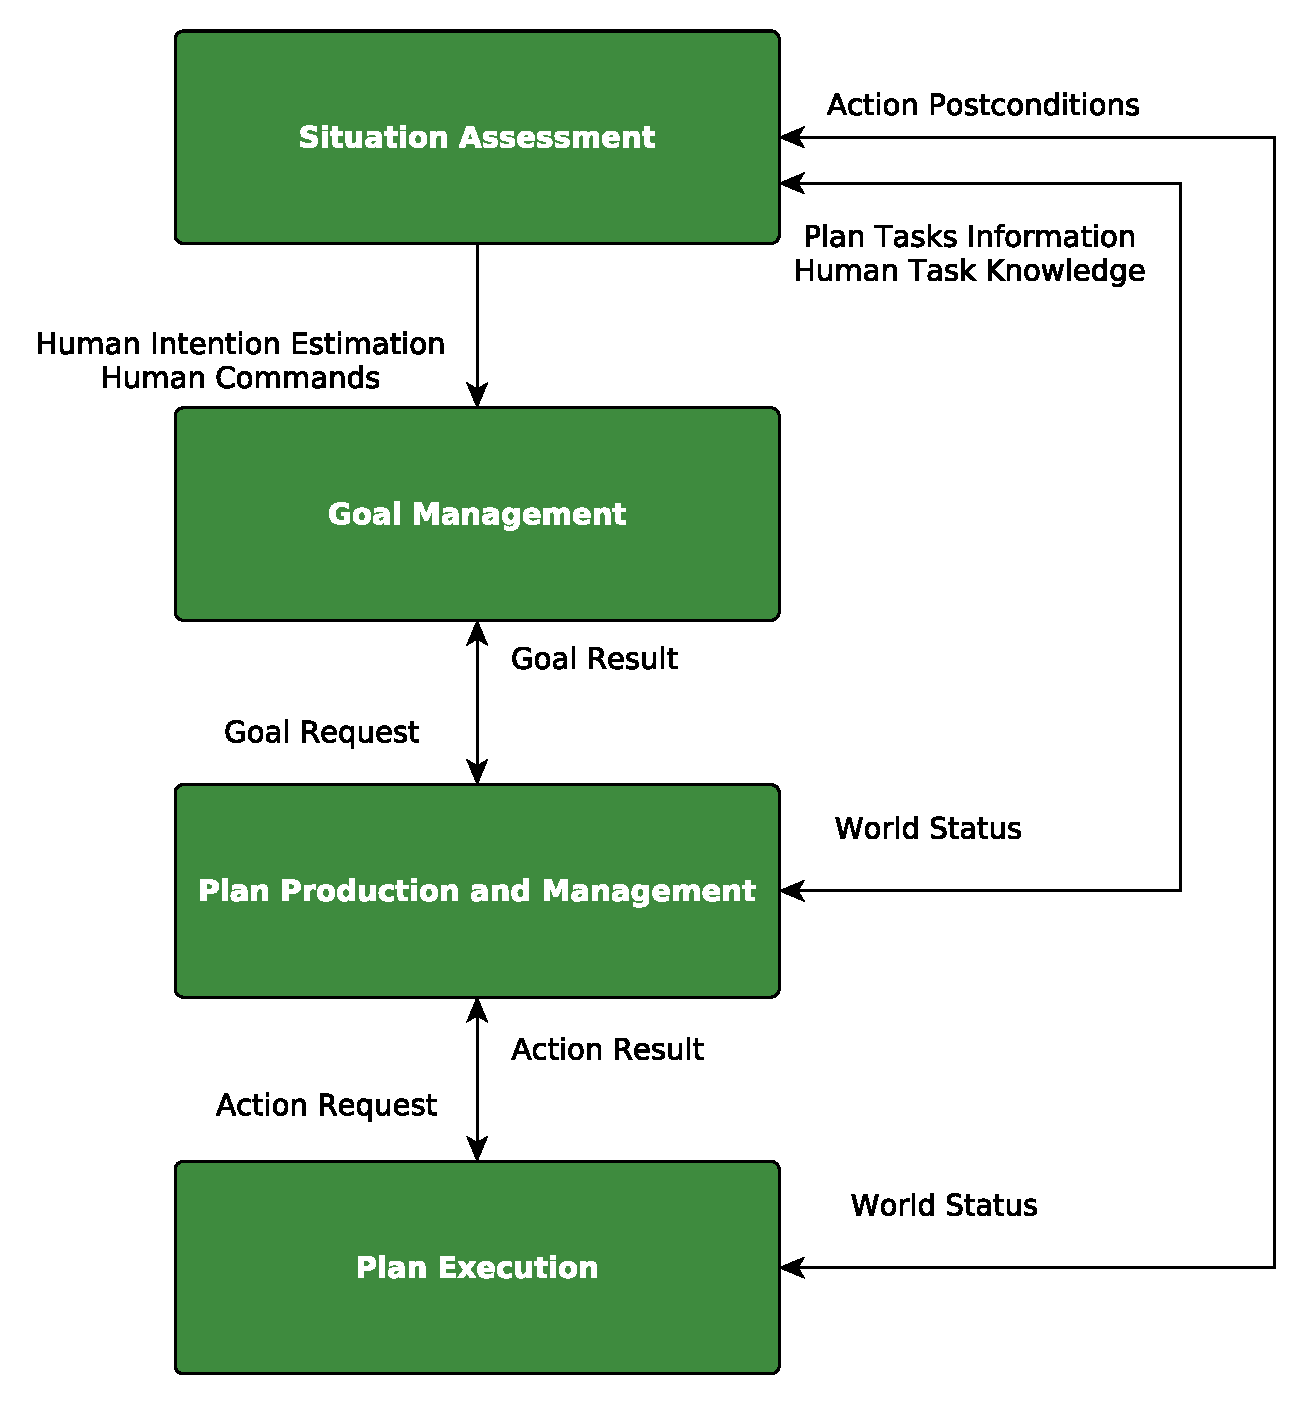
\includegraphics[scale=0.45]{img/intro/system_architecture}
	\caption{This picture shows the different layers of the system}
	\label{fig:intro-system_architecture}
\end{figure}

The system also interfaces itself with other modules, which can be easily changed depending on the current needs:

\begin{itemize}
\item Task Planner: this module is an abstraction for different Task Planner that can be used by the system. Different planners can be introduced in the system, by creating a new module that respects the conventions used by the Plan Manager.
\item Motion Planners:  this modules are used by the Execution Manager to plan the robot movements and actions. The system uses the Geometrical Task Planner (GTP) to plan manipulation actions and the well known Move Base stack for navigation planning. 
\item Motion Execution: this module executes trajectories planned by the Motion Planners. The system uses the Pr2Motion executor.
\end{itemize}

\section{Organization of the Thesis}

\section{Published Works}